\chapter{Introduction}\label{chap:intro}
This chapter introduces the assignment, along with some foundational concepts of quantum sensing. Furthermore, it covers the methodology, goals and boundaries, which all help outline the trajectory of the project.

\section{Background}\label{chap:background}
Quantum technology is become increasingly popular due to the promising practical solutions the once exclusively theoretical field of study is now producing. There are several research specialization within the field of quantum technology. Quantum computing is perhaps the most well-known, owing to its exploitation of quantum phenomena to solve previously incomputable, or nearly so, problems. Quantum communication is another prominent field, which has made significant . and quantum sensing. Out of the three, quantum computing is the focus of this project

\gls{nv} centers are imperfections in the atomic structure of diamonds \cite{enwiki:1301369588}. The two types of \gls{nv} centers are \gls{nv}0 and \gls{nv}-, as seen in Figure \ref{fig:nvcenter}, but the \gls{nv}- structure is much more commonly used in quantum applications. These imperfections have the useful property of spin-dependent luminescence. This means that the spin of the \gls{nv} center affects amount of light emitted by the structure\footnote{The \gls{nv} center only emits light after absorbing photons, a phenomenon called photoluminescence \cite{enwiki:1309081879}}. Using this quality of the \gls{nv} structure, different environmental metrics (e.g magnetic fields) can be measured. 

The Applied Nanotechnology research group is working on a \gls{nv}-center-based sensor setup, a high-level block diagram of which can be seen in Figure \ref{fig:overview_high_lvl}\footnote{Green blocks denote input/output (sub)systems, red blocks denote parts of the \gls{mw} system and blue blocks denote parts of the optical data path. This convention is used in other setup diagrams as well}. There exist several quantum protocols, but the one this setup needs to support is called \gls{cwodmr}. At its core, \gls{odmr} is a set of protocols, which can detect magnetic fields based on the changes in the fluorescence of quantum objects at specific frequencies (most commonly \gls{nv} centers) \cite{enwiki:1301371272}. \gls{cwodmr} in particular involves exposing the \gls{nv} center to a \gls{mw} frequency sweep while illuminating it with a constant light source. This is in contrast with \gls{podmr} techniques, which use different \gls{ttl} pulse schemes \cite{sewani2020coherent} to modulate the \gls{mw} signal and the light source. \gls{podmr} does not refer to a specific protocol, instead it denotes a family of quantum protocols. Out of all pulsed protocols, the Rabi oscillations protocol is the most important for the setup, as it is used for measuring high-frequency optical oscillations that form the base of quantum computing. Additionally, the $T_1$ measurements is also important, as it is used for measuring the $T_1$ relaxation time of the \gls{nv}[] centers and can be used for tuning Rabi oscillation experiments. Although \gls{cwodmr} is the main focus of the research group at the moment, support for pulsed protocols is also desired for future quantum  sensing and quantum computing research. 

\begin{figure}[ht]
	\centering
	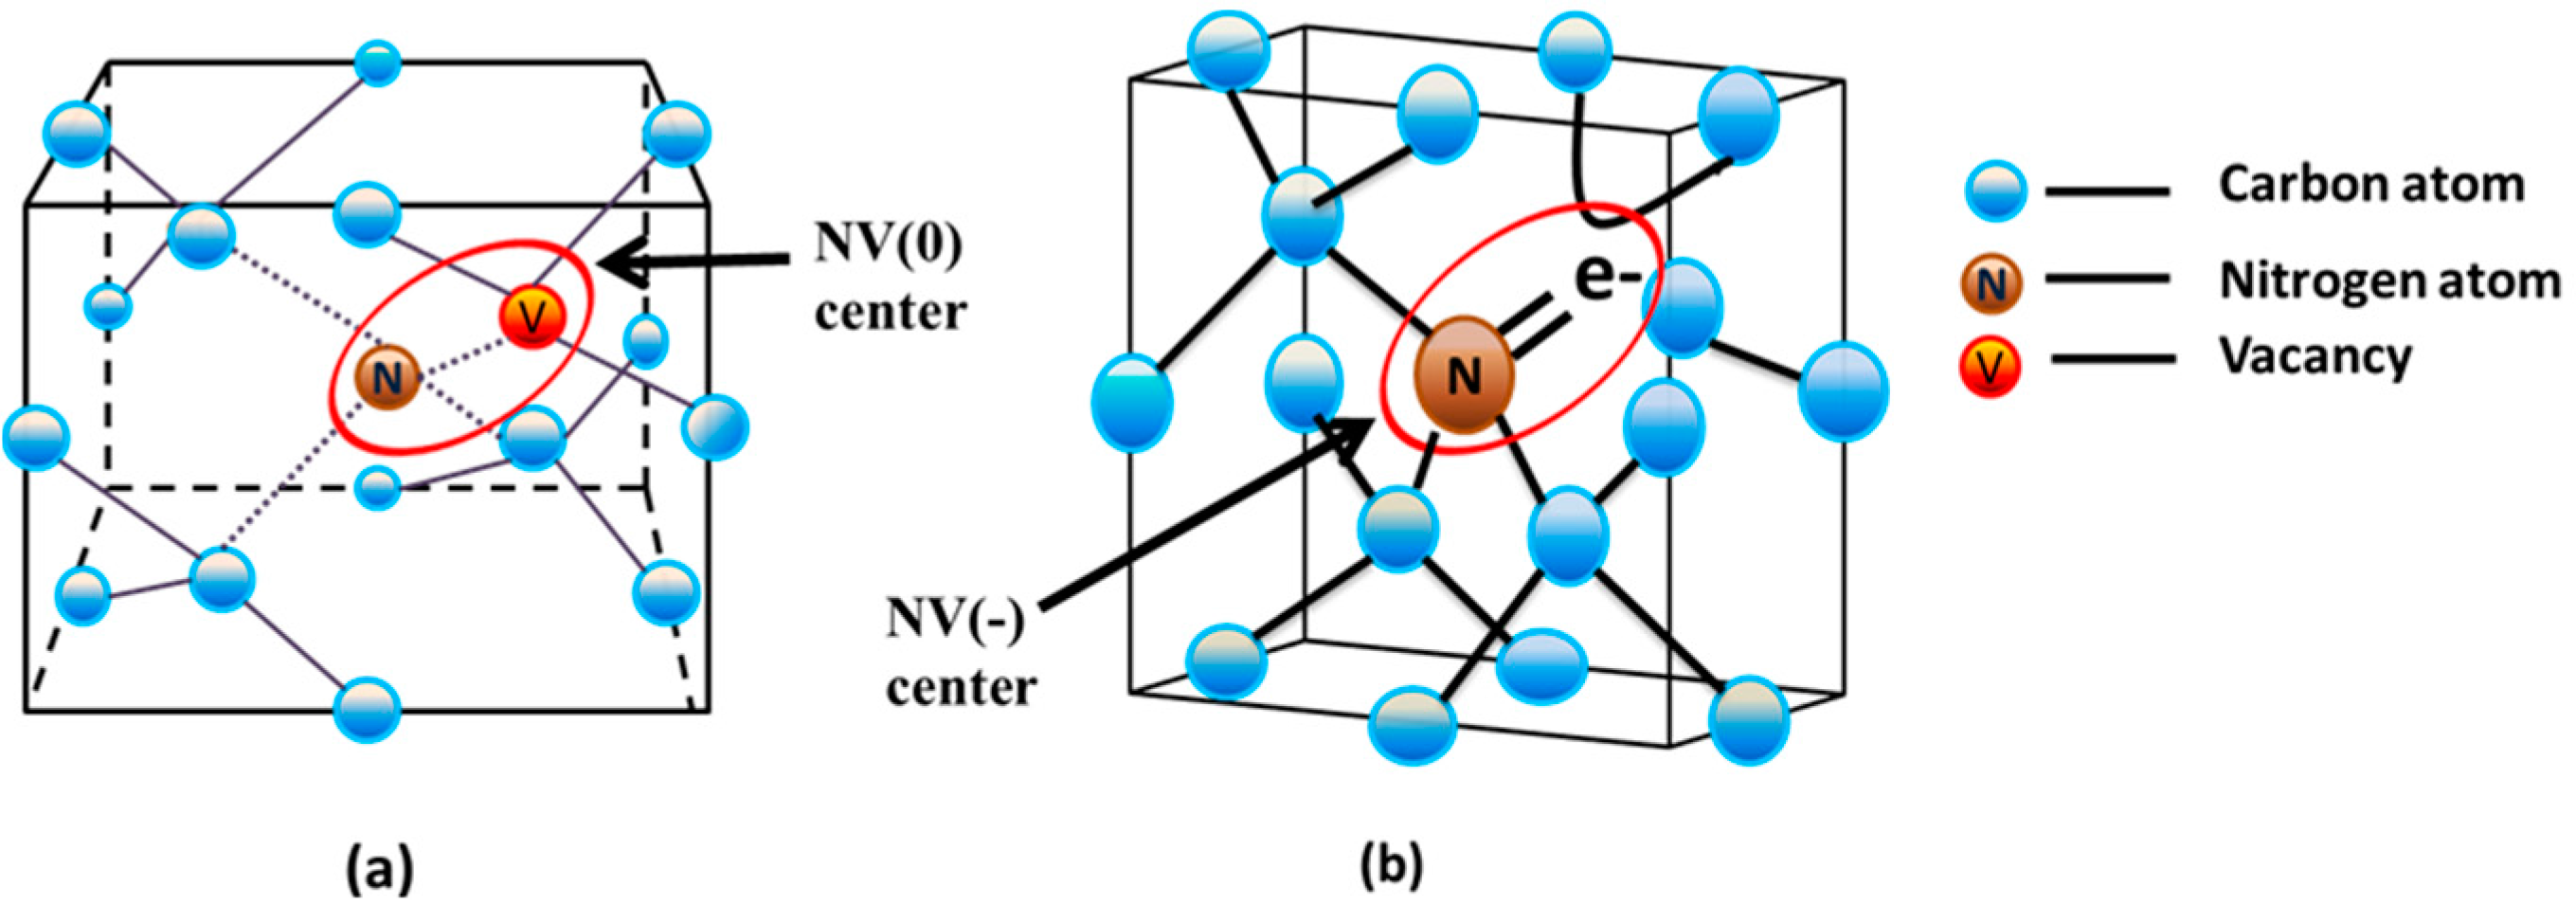
\includegraphics[width=0.7\linewidth]{img/nv_center}
	\caption{\gls{nv}0 (a) and \gls{nv}- (b) structures in diamonds (image credit to Haque et al \cite{haque2017overview})}
	\label{fig:nvcenter}
\end{figure}

Acquiring and processing data from the setup requires working with \gls{nv} fluorescence signals that are hard to distinguish from the laser light, because they are a total of 1-2 \% of the total signal. While this is a significant problem, it is also very common and there are existing solutions for low-intensity photodetection. This project is mainly about developing a similar system specifically for quantum sensing and the \gls{nv} setup, in particular. 


\begin{figure}[ht]
	\centering
	\begin{tikzpicture}[
		% define box styles
		boxr/.style={rectangle, thick, draw=red!50!black, fill=red!5, minimum size=5mm},
		boxg/.style={rectangle, thick, draw=green!50!black, fill=green!5, minimum size=5mm},
		boxb/.style={rectangle, thick, draw=blue!50!black, fill=blue!5, minimum size=5mm},
		]
		% draw MW nodes
		\node[boxg] (fgen)							{\textbf{Function generator}};
		\node[boxr] (mwsw)		[right=10 mm of fgen] 		{\glsfmtshort{mw} switch};
		\node[boxr] (mwant)		[right=of mwsw]		{\glsfmtshort{mw} antenna};
		\node[boxg] (mwsweep)	[above=of mwsw] 	{Frequency sweeper};
		% draw main system nodes
		\node[boxb] (driver) 	[below=of fgen]		{Current driver};
		\node[boxb] (laser) 	[below=of mwsw]		{Laser};
		\node[boxb] (nv) 		[below=of mwant] 	{NV sample};
		\node[boxb] (detect) 	[right=of nv]		{\textbf{Photodetector}};
		\node[boxg] (lockin)	[above=of detect]	{\textbf{\glsfmtshort{daq}}};
		
		
		% draw MW lines
		\draw[->, thick] 			(fgen.east) 		to node[midway, above]{Signal} 	(mwsw.west);
		\draw[->, thick] 			(mwsw.east) 		to node[midway, above]{Signal} 	(mwant.west);
		\draw[->, thick, dashed]	(mwsweep.south) 	to node[midway, left]{Sweep} 				(mwsw.north);
		% draw main system lines
		\draw[->, thick]			(fgen.south)		to node[midway, left]{Signal} 	(driver.north);
		\draw[->, thick] 			(driver.east) 		to node[midway, above]{Current} 			(laser.west);
		\draw[->, thick]			(laser.east) 		to node[midway, above]{Light} 				(nv.west);
		\draw[->, thick]			(nv.east) 			to node[midway, above]{Light}				(detect.west);		
		\draw[->, thick]			(detect.north) 		to node[midway, right]{Signal}				(lockin.south);	
		% draw long line
		\draw[->, thick, dashed] (fgen.south east) .. controls +(down:5mm) .. node[pos=.9, sloped, below]{Reference signal}(lockin.south west);
	\end{tikzpicture}
	\caption{High-level overview of the quantum sensing setup}
	\label{fig:overview_high_lvl}
\end{figure}

The setup diagram in Figure \ref{fig:overview_high_lvl} shows a complete setup overview, with the most important subsystems for this assignment highlighted. Neither \gls{cwodmr}[], nor $T_1$ measurements require all subsystems in order to operate. The specifics of how the setups is used to execute different quantum protocols are discussed in Chapter \ref{chap:intro:sequences}.

The most important setup subsystem specifically for this project is the \textbf{Photodetector} block, the implementation of which is the main priority of this assignment. It is the last part of the optical data path. Its purpose is to retrieve the optical signal, containing light from the laser and \gls{nv} centers, and output it to the \gls{daq} subsystem. When executing \gls{cwodmr}, the optical signal contains small and gradual changes in intensity, while the \gls{podmr} signal, as the name suggests, consists of a pulsed laser signal, as well as the resulting rapid fluctuations in \gls{nv} center luminescence.

Driving the laser at the beginning of the optical data path is done with the \textbf{Function generator}. Executing each protocols requires the automatic generation of either a constant signal or a pulse sequence (for more information, see Chapter \ref{chap:intro:sequences}). The frequency sweeper is the other input device and its only application is \gls{cwodmr} \gls{mw} sweeps (see Chapter \ref{chap:intro:cwodmr}). $T_1$ measurements do not require a microwave subsystem and Rabi oscillations need the \gls{mw} signal to be pulsed by the \textbf{Function generator} again.

In addition, the system also needs the raw signal from the photodetector to be extracted by the \textbf{\gls{daq}} subsystem. Data acquisition for \gls{cwodmr} is simple, only requiring an analog-to-digital signal conversion before experiment data can be stored. However, when a pulsed protocol experiment is being carried out, a \gls{lia} (see Chapter \ref{chap:lockin}) needs to be used to extract the photoluminescent signal at specific frequencies.



\section{Purpose of the assignment}\label{purpose}
The main purpose of the assignment is to implement one photodetector specifically for \gls{cwodmr} and another for \gls{podmr}. Commercial solutions, while very sensitive, cannot be used due to their high cost and physical size. The quantum sensing setup is made up of other systems as well, which is why there are also several additional functionalities and systems that need to be developed, in order for the setup to support quantum magnetometry.


For experiments to be carried out, a data acquisition system has to be implemented. Acquiring data will be done with the use of the \gls{ad2}\footnote{The \gls{ad2} is a multi-functional electronic instrument. It provides oscilloscope capabilities and an analog waveform generation pipeline, among other functionalities.}, as requested by the client. In the same vein, the client has asked that the \gls{ad2} be used for generating \gls{podmr} pulsing sequences. These sequences are used to drive the various subsystems of the sensor during an experiment. For more information about pulsing sequences, see Chapter \ref{chap:intro:sequences}. The reason the client has requested the use of this particular device is that its compact size and various functionalities make it an enticing all-in-one option for handling system input and output. The perks of using the \gls{ad2} is that it is relatively inexpensive, small and can simplify the code base by removing the need for multiple input/output devices. Both sequence generation and data acquisition need to be automated in order to simplify the experiment workflow. To make the operation of the quantum sensor even more straightforward, a \gls{gui} has to be implemented as well. Its primary purpose is to combine sequence generation and data acquisition in the same software solution, while keeping the front end clean and straightforward for the convenience of the sensing setup user. Additionally, the software should be modular enough to facilitate further development in the future.


\section{Assignment specifications}\label{specifications}
As already explained, the assignment is quite broad and involves both hardware and software, causing the need for a number of different tools, which are described in this section.

Most of the hardware tools are already available at the Applied Nanotechnology lab. Most important of all is the equipment used for debugging the photodetector. Current and voltage supplies, along with oscilloscopes for measuring output, can be used to verify the working of the system.

In order to get an operational \gls{cwodmr} setup, a \gls{mw} generator and a laser will be used. \gls{mw} sweeping needs to be done in the range of \numrange{2,8}{2,9} \unit{\giga\hertz} and the lab already has a custom-built \gls{mw} generator that can output these frequencies. Chapter \ref{chap:intro:cwodmr} covers the rest of the background information about \gls{cwodmr}.

Pulsed protocols use the same hardware as \gls{cwodmr}, but they utilize it differently. Instead of sweeping through frequencies with the \gls{mw} generator and keeping the laser constantly on, the $T_1$ measurements protocol requires the laser to send out 5 \unit{\micro\second} pulses, without needing the \gls{mw} generator. The Rabi oscillations protocol is more involved, as it requires both laser and \gls{mw} pulsing with different timings (see Chapters \ref{chap:fd:t1} and \ref{chap:fd:podmr}). It also has higher frequency requirements than $T_1$ measurements, because the optical effect of the oscillations has a frequency of \numrange{3,2}{4} \unit{\mega\hertz} \cite{murzakhanov2025mechanism}. Both protocols need a \gls{lia} to extract the desired signal from the noisy system output, so the Zurich Instruments HF2LI will be used for that purpose.

Crucially, \gls{cwodmr}[] photodetection differs significantly from \gls{podmr}[] photodetection. At their core, the two types of protocols have different photodetector requirements. A \gls{cwodmr}[] sensor needs the noise to be as low as possible, because it should not use a \gls{lia}, but it can work with a narrow-bandwidth photodetector \cite{acharya2025compact}. Pulsed protocols, on the other hand, all involve high-frequency optical signals, which require a broad bandwidth for proper detection. Consequently, a \gls{podmr}[] sensor cannot work without a \gls{lia}, but because of this, the noise requirements are much more lax.

The laser itself is mostly outside the scope of the assignment, as its application is almost entirely optical in nature. However, driving the laser is important for the working of the setup and the testing of the photodetectors. The driving circuitry has been developed by a previous intern, but integration with the photodetectors will be carried out in this project. The driver will be fed \gls{ttl} pulse data from an \gls{ad2}-based waveform generator. It is important to note that the fluorescence wavelength is in the range of \numrange{637}{800} \unit{\nano\meter} \cite{hsiao2016fluorescent, enwiki:1301371272}. It is different from the laser wavelength of 518 \unit{\nano\metre}, which is filtered out and is not supposed to be detected by the photodetector. Lastly, FabLab equipment can be used when a tool is not available at the quantum lab. 
	
In terms of software, there is more freedom of choice. Interfacing with the HF2LI is done through proprietary software. Similarly, pulse generation and data acquisition has to be done with Waveforms and its \gls{api}, but those are the only programs that cannot be replaced. The program for retrieving data from the data acquisition system can be written in both Python and MATLAB. Both languages support the necessary \gls{api}s. They also offer \gls{gui} programming capabilities and are good for scientific computing in general. Python has the advantage of being open-source and free.

Theoretical models of the developed systems will be computed using MATLAB, because of the variety of tools it offers for electronic design and scientific computing. LTSpice and Tina-TI will both be used for \gls{spice} simulations of circuit designs, depending on what hardware is being simulated, as both offer simulations more in line with real devices than the mathematical models. As for \gls{ecad} software, there are various suites that offer the same base functionality. KiCad was selected because the client prefers open-source software.  



\section{Scope of work}
The scope of the project was extensively discussed with the company coach. Chapter \ref{chap:project_boundaries} sets the project boundaries and Chapter \ref{chap:goals} builds on them, providing more specific details.

\subsection{Project boundaries}\label{chap:project_boundaries}
% specify what moscow is and put it in front of the goals
The project boundaries were initially based on the assignment form, but were later discussed with the client and refined further. 

\textbf{Must have}
\begin{itemize}
	\item Hardware platform for \gls{cwodmr} photodetection
	\item Hardware platform for \gls{podmr} photodetection
%	\item Setup integration
\end{itemize}

\textbf{Should have}
\begin{itemize}
	\item \gls{podmr} sequence generation
	\item \gls{podmr} data acquisition
	\item \gls{gui} application
\end{itemize}

\textbf{Could have}
\begin{itemize}
	\item Setup integration
\end{itemize}

\textbf{Will not have}
\begin{itemize}
	\item All-in-one detection platform with the laser as a part of the photodetector \gls{pcb}
	\item Laser driver upgrade
\end{itemize}


\subsection{Goals} \label{chap:goals}
% goals are tasks now, change to goals
Based on the MoSCoW priorities from Chapter \ref{chap:project_boundaries}, a set of goals and tasks was created to further specify all items from each prioritization category. Every task was designed so that its outcome is a tangible project milestone (e.g. code or hardware).

\begin{itemize}
	\item[Goal 1]: Create two hardware setups, one for \gls{cwodmr}[] and one for \gls{podmr}[], which measure and amplify photodiode signals 
	\item[Goal 2]: Develop software to drive the laser and process lock-in amplifier signals
	\item[Goal 3]: Begin hardware and software integration
\end{itemize}

While these goals are practical, they are still not specific enough. To eliminate the possibility of confusion, a set of tasks were created. All tasks contribute to one of the three goals.

\begin{itemize}
	\item[Task 1.1]: Design a photodetector \gls{pcb} for \gls{cwodmr}
	\item[Task 1.2]: Design a photodetector \gls{pcb} for \gls{podmr}
	\item[Task 2.1]: Program quantum protocol pulse sequences for $T_1$ measurements 
	\item[Task 2.2]: Develop software that acquires the system output
	\item[Task 3.1]: Test photodetector with laser
	\item[Task 3.2]: Create a \gls{gui} that encapsulates data acquisition and sequence generation for \gls{podmr}
\end{itemize}

\textbf{Task 1.1} involves the design and production of a photodetector \gls{pcb} to handle the \gls{cwodmr} protocol in particular. It was decided that the initial design of the board should consist of a \gls{tia} that amplifies the current generated by the Vishay BPW34 photodiode. This circuit needs to work with the quantum sensing setup, but also with a portable sensing setup, which is currently in development. The \gls{tia} needs to have a gain of 160 \unit{\decibel}, but no bandwidth requirement is set, because \gls{cwodmr}[] measurements have been done with a bandwidth as narrow as 18 \unit[]{\hertz} \cite{acharya2025compact}. However, as a result of the fluorescence of the \gls{nv} centers being around \numrange[]{1}{2} \% of the total optical signal, the photodetector has to have low noise. After consulting both literature \cite{chuprina2026impact} and Applied Nanotechnology researchers, it was decided that the spectral noise density of the \gls{tia} should be reduced as much as possible and that it should not exceed 5 \unit[power-half-as-sqrt]{\micro\volt\per\hertz\tothe{0.5}}. A holistic approach needs to be taken when investigating the system noise, however it is also important that the different noise components are investigated separately. Even though the final noise figure at the system output is most important, the flicker noise, thermal noise and shot noise need to be accounted for. In addition to fulfilling all technical requirements, the board should also be affordable. No concrete price point has been set, though the price board should definitely not exceed 50 \texteuro. Lastly, the physical board has to adhere to the Thorlabs photonics mounting standard. This hardware platform has the highest priority, which is why it will be implemented first.

\textbf{Task 1.2} is to develop a photodetector for pulsed quantum sensing protocols, more specifically $T_1$ measurements and Rabi oscillations, with other pulsed protocols also being considered for future implementation. Some of the requirements overlap with those from \textbf{Task 1.1}, namely the use of the BPW34, the 160 \unit[]{\decibel} gain and the dimensions of the \gls{pcb}. That being said, the two photodetectors are noticeably different. The \gls{podmr} sensor needs a wide bandwidth, due to the high-frequency optical signals generated by pulsed protocols. Rabi oscillations is the protocol that determines the bandwidth, as the optical fluctuations that need to be measured have a sinusoidal shape and are in the range of \numrange{3,2}{4} \unit{\mega\hertz} \cite{murzakhanov2025mechanism}. To guarantee that the bandwidth is sufficient to measure the oscillations, the cutoff frequency needs to be at least 5 \unit{\mega\hertz}. While the \gls{cwodmr}[] \gls{pcb} takes precedence over the \gls{podmr}[] \gls{pcb}[], the similar hardware used in both means there can be some task parallelization when designing and testing the circuits, so working on both can be done in the same time frame.

\textbf{Task 2.1} involves the programming of pulsing sequences for pulsed protocols. Automatic generation of $T_1$ measurements sequences is the primary objective of this task. At least 25 sequences with variable dark time (see Chapter \ref{chap:fd:podmr}) need to be generated. The sequences should be based on the ones presented in Sewani et al \cite{sewani2020coherent}, though the timings might need to be scaled, due to differences in the physical experiment setup. Automation has to be done with the Waveforms \gls{api} in either Python or MATLAB, because of the use of the \gls{ad2} waveform generator. Having pulsing sequences, even if their generation is not automated is a prerequisite for starting the next task. Consequently, they should be developed before moving on to \textbf{Task 2.2}. 

\textbf{Task 2.2} requires the programming and automation of the \gls{ad2} oscilloscope. Acquiring data using the device has to be done with the Waveforms \gls{api}, with the interfacing code either written in Python or MATLAB. The desired result is a user-friendly method for acquiring data while doing $T_1$ measurements. In this task, the focus is on handling the microsecond timings (e.g. 5 \unit{\micro\second} laser pulses) and preserving the pulse shape, which is why $T_1$ was singled out for implementation. Despite developing a solution for a single protocol, the code should be as modular as possible to allow for protocol support to be extended in the future. As all coding activities are secondary to making the photodetector, this task should be completed after the first two tasks. Additionally, $T_1$ pulsing sequence are required to test the data acquisition, so the previous task needs to be completed before starting this one. Bridging the two tasks with the shared use of the \gls{ad2} is desired in order to provide a compact and affordable all-in-one solution for handling system input/output.

\textbf{Task 3.1} can only be started after the implementation phase of the V-Model (see Chapter \ref{methodological_approach}). The photodetectors and their integration with the laser driver have to be tested using a systematic approach. Each design iteration should undergo the same testing and, if a new design has to be made, it should be based on the test results. 

\textbf{Task 3.2} is similar to \textbf{Task 3.1}, except its focus is on software integration. A \gls{gui} that encapsulates the data acquisition and waveform generation needs to be programmed. This can be done with the help of TKinter (Python) or App Designer (MATLAB), as they are the simplest \gls{gui} creation tools in their respective language. As mentioned in Chapter \ref{specifications}, Python has the advantage of being open-source, which is why it is preferred, unless specific circumstances make its use impossible. Because of the differences in protocols, the application only needs to handle $T_1$ measurements, though code modularity is also expected. Additionally, the user should have the freedom to change the parameters of the experiment. Nevertheless the front end should be simple and intuitive. This task has the lowest priority, because its completion is not a mandatory prerequisite for any other task and, as a consequence, it should be done last.


\subsection{Deliverables}
The description of the tasks already provided context for the deliverables, but this subsection contains a formalized version of the deliverables.

\begin{enumerate}
	\item Photodetection \glspl{pcb}
	\item Data acquisition routines
	\item Pulsing sequences
	\item \gls{gui} application
	\item Technical documentation
\end{enumerate}

The only deliverable, which was not mentioned in Chapter \ref{chap:goals} is the technical documentation. This is because it should contain information about every task.

\section{Methodology}\label{methodological_approach}
\begin{figure}[ht]
	\centering
	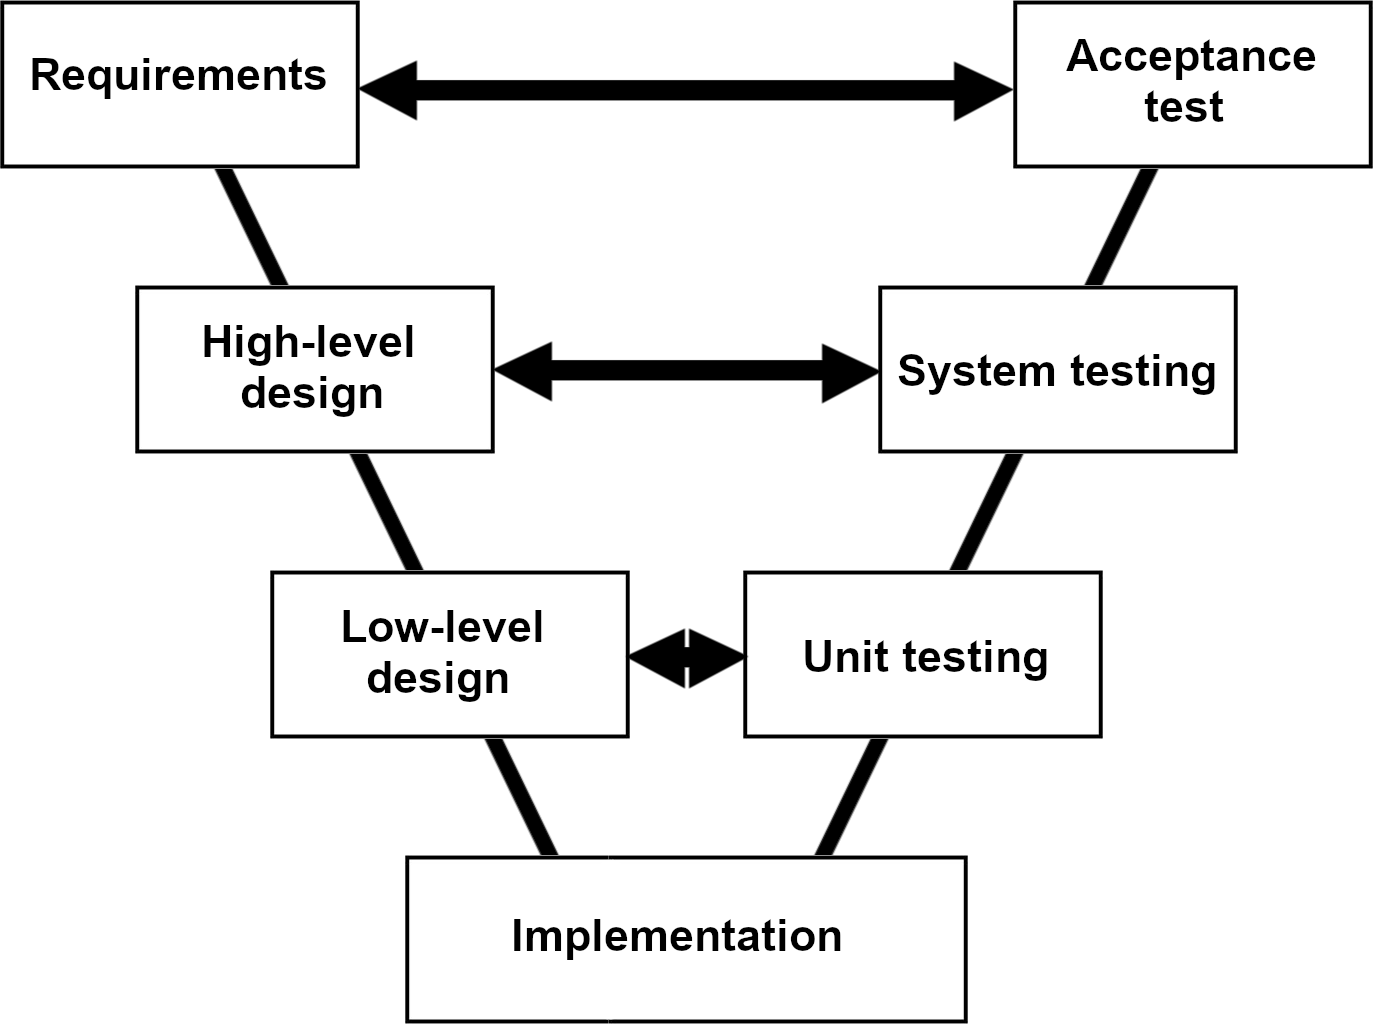
\includegraphics[width=0.7\linewidth]{img/vmodel}
	\caption{V-Model diagram}
	\label{fig:vmodel}
\end{figure}

The V-Model methodology was selected, as it is well-suited for hardware and low-level software projects. Figure \ref{fig:vmodel} shows a diagram of the phases of the V-Model. Unlike some software-oriented models, the V-Model is very sequential. This can sometimes be seen as detrimental, but in this case it helps with structuring the project. Another benefit of this model is that there are multiple testing activities underpinning the quality assurance. A contentious feature of the V-Model is the heavy reliance on the initial requirements. This need for deliberate project requirements can be hard to meet, especially if the client representative is not technically proficient. In this project, the requirements were extensively discussed with the representative of the Applied Nanotechnology research group, who is an experimental physicist. Based on the discussion, the project boundaries in Chapter \ref{chap:project_boundaries} were set up.



\section{Report outline}
The introduction is followed by the functional design chapter, which introduces background knowledge, needed to understand the \gls{nv} setup. After that, the high-level design of the system is presented. It explains the functionality of the various systems that make up the project without delving into specifics.

After that, the technical design explores the low-level design of the systems of the project. It mentions all the necessary details, including calculations, simulations and implementation steps.

Following the design sections, the testing chapter describes the testing goals and what methods were used for measuring. The chapter then presents the test results, followed by a short discussion of what they mean for the photodetector and the setup as a whole. 

Lastly, the conclusion and recommendation chapters summarize the outcomes of the project and offer proposals for further development. 